\section{Evaluation}

\begin{itemize}
  \item what question our evaluation answers and why?
\end{itemize}

\subsection{Simulation}
Synthetic users simulation to evaluate FairTest reports.

\begin{figure*}[t]
{
  \subfigure[Income]{
    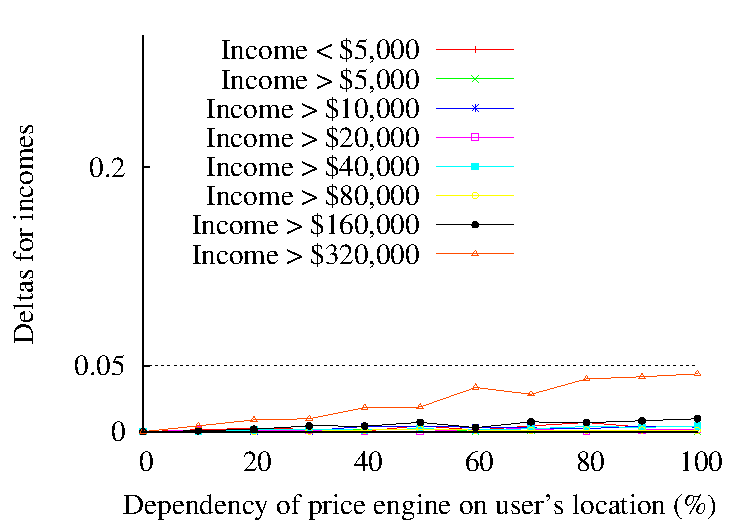
\includegraphics[width=0.33\textwidth]
    {\detokenize{results/income_discrimination_on_location_dependency}}
    \label{fig:}
 }
 \subfigure[Race]{
    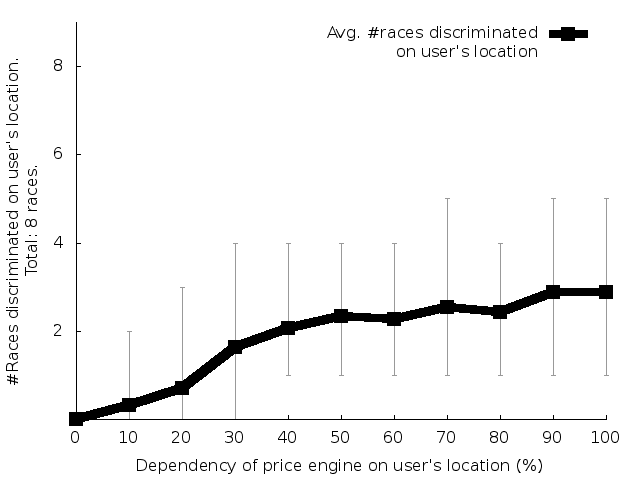
\includegraphics[width=0.33\textwidth]
    {\detokenize{results/race_discrimination_on_location_dependency}}
    \label{fig:}
  }
 \subfigure[Sex]{
    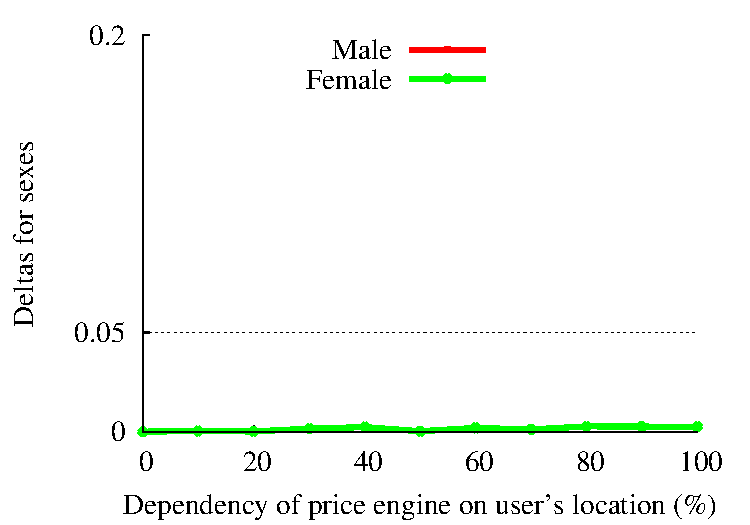
\includegraphics[width=0.33\textwidth]
    {\detokenize{results/sex_discrimination_on_location_dependency}}
    \label{fig:}
  }
 \caption{\textbf{Statistical parity and its dependency on user's location.}
          Shows the dependency of statistical parity, i.e., number of samples that
          violate condition~\ref{eq:StatisticalParity}, as a function of (a) user's income,
          (b) user's race, and (c) user's sex. Figure (b) reveals that statistical parity on
          user-incomes correlates with the dependency of the price engine on user's location.
          While Figures (a) and (b) reveal that statistical parity on user-race and on user-sex
          do not correlate with the dependency of the price engine on user's location.}
}
\end{figure*}


\begin{figure*}[t]
{
  \subfigure[Income]{
    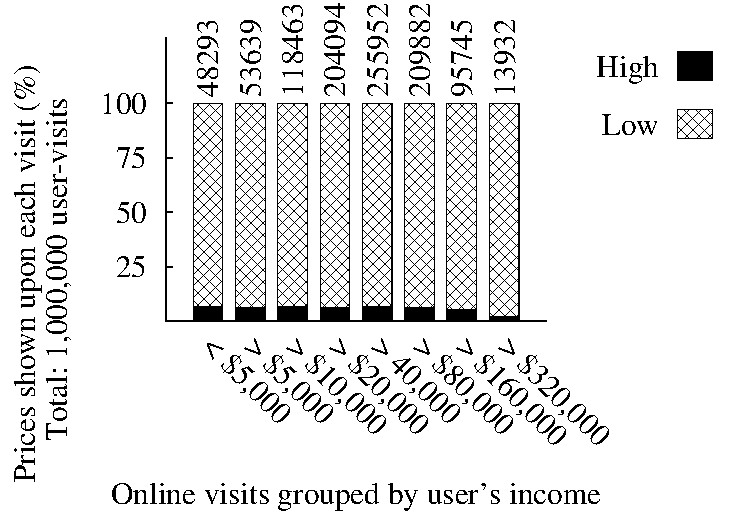
\includegraphics[width=0.33\textwidth]
    {\detokenize{results/income_discrimination_on_proportional}}
    \label{fig:IncomeDiscriminationProportional}
 }
 \subfigure[Race]{
    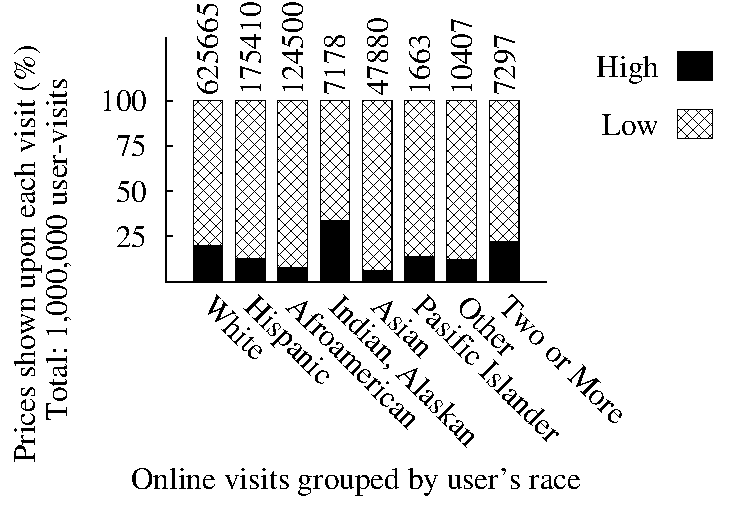
\includegraphics[width=0.33\textwidth]
    {\detokenize{results/race_discrimination_on_proportional}}
    \label{fig:}
  }
 \subfigure[Sex]{
    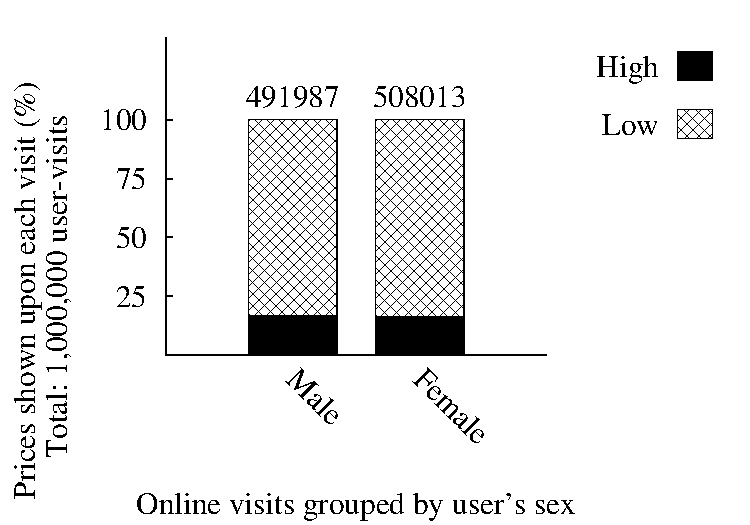
\includegraphics[width=0.33\textwidth]
    {\detokenize{results/sex_discrimination_on_proportional}}
    \label{fig:}
  }
 \caption{\textbf{Prices shown to users and their dependency on income, race, and sex.}
          Shows the proportion of high versus low prices shown to users based on income,
          race, and sex. Figure (a) reveals that a users with annual income less than
          \$5,000 receive proportionaly more high prices than users with annual income
          more than \$320,000. Figure (b) indicates that Indian or Alaskan users receive
          notably more high prices than any other race. This raises a consern, since as
          shown in Figure~\ref{fig:IncomePerRace}, an Indian or Alaskan user has a
          considerably lower income than a white American user. Figure (c) shows that
          male and female users receive approximately the same proportion of high versus
          low prices.}
}
\end{figure*}


\begin{figure}[!h]
 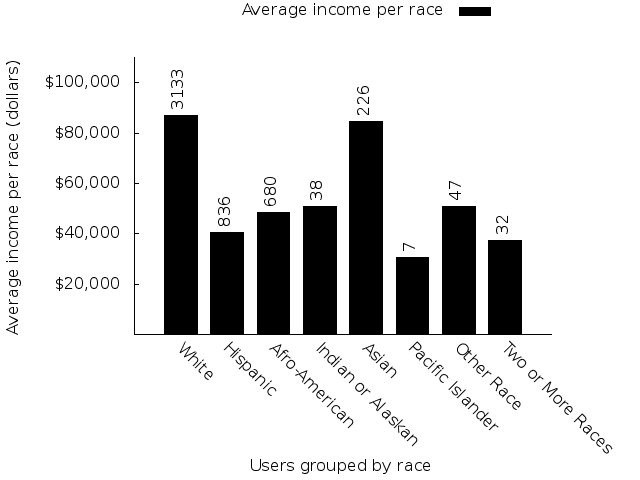
\includegraphics[width=0.49\textwidth]
  {\detokenize{results/income_per_race}}
  \caption{\textbf{Average user income for each race.} An Indian or Alaskan user has
           a considerably lower income than a white American user, and yet, as shown in
           Figure~\ref{fig:IncomeDiscriminationProportional}, he or she receives
           proportional more high prices compared to a white American.}
  \label{fig:IncomePerRace}
\end{figure}
